\section{Optymalizacja przy użyciu pakietu JModelica.org}
\label{sec:opt}

Podstawowym zadaniem wyższego poziomu aplikacji było przeprowadzenie optymalizacji w celu wyznaczenia sterowania czasooptymalnego. Jak wspomniano w sekcji \ref{sub:czesc-wyzsza-wybor}, wybrano do tego celu platformę JModelica.org.

%-------------------------------------------------
\subsection{Opis algorytmu optymalizacji dynamicznej}
\label{sub:opt-alg}

Algorytm wykorzystywany do optymalizacji dynamicznej można ogólnie opisać jako bezpośrednią metodę kolokacji. Polega ona na aproksymacji układu równań różniczkowych w dyskretnych chwilach czasu i konstrukcji na tej podstawie zadania programowania nieliniowego, zwykle o rzadkiej strukturze. Jest napisana w języku Python i używa biblioteki CasADi do wyznaczenia wartości pochodnych funkcji oraz oprogramowania IPOPT do obliczenia wynikowego zagadnienia programowania nieliniowego. Można z niej korzystać pod warunkiem, że model matematyczny nie zawiera nieciągłości (za: \cite{JModelicaUserGuide}). W związku z tym, że w rozważanym modelu układu zbiorników występuje osobliwość dla zerowego poziomu w trzecim zbiorniku, należało unikać trajektorii zawierających ten punkt.
Rzeczywiście, przy próbie uruchomienia optymalizacji dla warunku początkowego niedaleko tego punktu, algorytm zwracał błąd niepoprawnej wartości pochodnej.
Nie można więc stosować tego algorytmu do napełniania zbiorników od stanu zerowego, co zmniejsza jego praktyczne zastosowanie.

Programy rozwiązujące problemy NLP wykazują się dużo większą zbieżnością w przypadku, gdy dostarczy się im informacje o pochodnych pierwszego i drugiego rzędu (za: \cite{and+11mod11}). W związku z tym w użytym algorytmie użyto najpierw oprogramowania CasADi, aby ze skompilowanego modelu w języku Modelica wyznaczyć wartości tych pochodnych (w formie jakobianu), a następnie używa się metody elementów skończonych. Dzieli ona wejściowy czas działania na określoną liczbę przedziałów nazywanych elementami skończonymi i dostarcza aproksymacji nieznanych wartości sterowania i stanów systemu w określonej liczbie punktów kolokacji. Wpływ liczby elementów na jakość rozwiązania jest przedstawiony w sekcji \ref{sub:sym-wer-jmodelica}.
W każdym punkcie kolokacji zastosowano pakiet IPOPT, który rozwiązuje zadanie w postaci danej wzorem \ref{eq:opt-stat} za pomocą metody punktu wewnętrznego. Metoda ta wykorzystuje funkcję graniczną do poruszania się tylko wewnątrz zbioru dopuszczalnego, gdzie metodą Newtona szuka lokalnego minimum.

\begin{equation}\label{eq:opt-stat}
    \min\limits_{x \in [x_{l}, x_{u}]~ \land~ g_{l} \leq g(x) \leq g_{u}} f(x)
\end{equation}

Algorytm optymalizacyjny zwraca wektor sterowań oraz trajektorie układu w czasie będącym wartością wskaźnika jakości w tym zagadnieniu. Te wartości są prezentowane użytkownikowi jako odpowiednie atrybuty urządzenia systemu Tango Controls.

Brak uwzględnienia ograniczenia czasu końcowego $T \geq 0$ w niektórych przypadkach skutkowało znalezieniem sterowania z ujemnym czasem optymalnym. Wynika z tego, że opisana metoda nie jest wrażliwa na to, że symuluje fizyczny układ, co może dziwić, zważywszy na fakt, iż została napisana dla oprogramowania służącego tylko do symulacji.
To ograniczenie zostało uwzględnione w definicji optymalizacji w języku Optimica, które pokazano w sekcji \ref{sub:czesc-wyzsza-wybor}, aby uniknąć pojawiania się ujemnego czasu optymalnego.

%-------------------------------------------------
\subsection{Inicjalizacja optymalizacji dynamicznej}
\label{sub:opt-init}

Kluczowym aspektem funkcjonowania algorytmów optymalizacji dynamicznej jest odpowiednie określenie punktu początkowego, czyli początkowej struktury sterowania i wygenerowanej przez nią trajektorii układu. Jest to zagadnienie szeroko opisywane w literaturze, m.in w \cite{Betts98}, \cite{Rao2010}, \cite{Korytowski2015}, \cite{cas+11ifac} oraz \cite{JModelicaUserGuide}.
Początkowo próbowano inicjalizować algorytm stałym sterowaniem, którego wartość jest niezależna od punktów początkowych i końcowych. Niestety, takie podejście okazało się błędne i nie udało się wyznaczyć żadnego sterowania optymalnego.

W związku z tym przyjęto następujący algorytm inicjalizacyjny:
\begin{itemize}
    \item dla każdej z trzech wartości poziomów docelowych wyznacz wartość sterowania ustalonego na podstawie odwrotności wzoru \ref{eq:model-steady-state} danego wzorem \ref{eq:steady-ctrls},
    \begin{equation} \label{eq:steady-ctrls}
    u_{i} = C_{i}h_{i}^{\alpha_{i}}
    \end{equation}
    \item wyznacz wartość średnią z trzech sterowań ustalonych, wyznaczonych w poprzednim kroku według wzoru \ref{eq:steady-ctrl}
    \begin{equation}\label{eq:steady-ctrl}
    u_{r} = \frac{1}{3} \cdot \sum_{i=1}^{3} u_{i}
    \end{equation}
    \item przeprowadź symulację z czasem końcowym podanym jako wartość właściwości \emph{SimulationFinaltime} (opisanej w sekcji \ref{sub:czesc-wyzsza-klasa}),
    \item podaj wyniki uzyskane w symulacji jako trajektorie inicjalizacyjne do algorytmu optymalizacji.
\end{itemize}

\begin{figure}[ht]
    \centering
    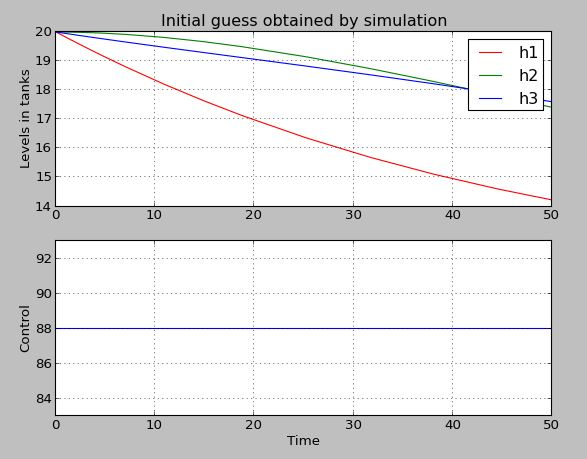
\includegraphics[scale=0.9]{Grafika/initial_guess}
    \caption{Przykładowa trajektoria początkowa dla algorytmu optymalizacji. Źródło: własne.}
    \label{fig:initialguess}
\end{figure}

Rysunek \ref{fig:initialguess} przedstawia przykładowe sterowanie ustalone i przebiegi zmiennych stanu uzyskane według powyższego algorytmu.


%-------------------------------------------------
\subsection{Uzyskana postać sterowania}
\label{sub:opt-ctrl-form}

W związku z tym, że użyte oprogramowanie jest w stanie dokonywać optymalizacji sterowania w układach nieliniowych, nie ma możliwości, aby ograniczyć postać sterowania tylko do postaci ,,bang-bang''. Sterowanie wyznaczane przez opisany wyżej algorytm optymalizacji jest wektorem o liczbie elementów danej wzorem \ref{eq:ctrl-len}, gdzie $k$ to liczba punktów kolokacji, a $e$ to liczba elementów skończonych. Dodatkowy element wektora sterowania bierze się od wartości początkowej.

\begin{equation}\label{eq:ctrl-len}
l_{u} = k \cdot e + 1
\end{equation}

Niezależnie od tego okazało się, że sterowanie optymalne wyliczone przy pomocy pakietu JModelica.org ma postać zbliżoną do ,,bang-bang'' ze spodziewaną liczbą dwóch przełączeń. Dowodzi to, iż założenie opisane w sekcji \ref{sub:toc-nonlnr} jest prawdziwe, przynajmniej dla tych stanów początkowych i docelowych, dla których udało się wyznaczyć poprawnie sterowanie optymalne w ramach testów prowadzonych na potrzeby niniejszej pracy.

\begin{figure}[ht]
    \centering
    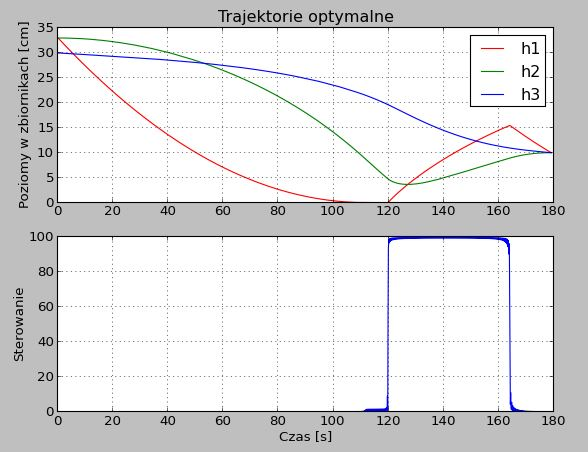
\includegraphics{Grafika/optimisation_example}
    \caption{Przykładowy wynik optymalizacji. Źródło: własne.}
    \label{fig:optimisationexample}
\end{figure}

Rysunek \ref{fig:optimisationexample} przedstawia przykładowe sterowanie optymalne oraz trajektorie układu przez nie wygenerowane. Można na nim zauważyć, że sterowanie nie jest dokładnie postaci ,,bang-bang'', ale jest to niego zbliżone.

Przyjęto więc prostą metodę normalizacji sterowania do postaci ,,bang-bang'': każdemu punktowi powyżej połowy różnicy między ograniczeniami nałożonymi na sterowanie zostaje przypisana wartość maksymalna, a każdemu poniżej - minimalna. Jeśli występuje tylko jeden czas przełączenia, to dodaje się drugi w ostatniej chwili czasu optymalizacji, a więc w momencie odpowiadającym wartości czasu optymalnego.
Taka operacja pozwala wyznaczyć czasy przełączeń potrzebne niższemu poziomowi aplikacji, jeśli tylko sterowanie otrzymane z algorytmu optymalizacji ma spodziewaną strukturę. Przykład działania operacji normalizacji jest dany poniżej: przedstawiono sterowanie w postaci ,,surowej'' obliczonej przez algorytm optymalizacyjny i po normalizacji odpowiednio na rysunkach \ref{fig:ctrl-raw-example} i \ref{fig:ctrl-normalised-example}.

\begin{figure}[ht]
    \centering
    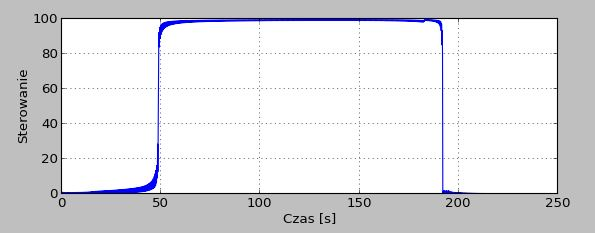
\includegraphics[width=\textwidth]{Grafika/ctrl_30_30_30-20_25_20-raw}
    \caption{Przykład sterowania ,,surowego'' otrzymanego w wyniku optymalizacji. Źródło: własne.}
    \label{fig:ctrl-raw-example}
\end{figure}

\begin{figure}[ht]
    \centering
    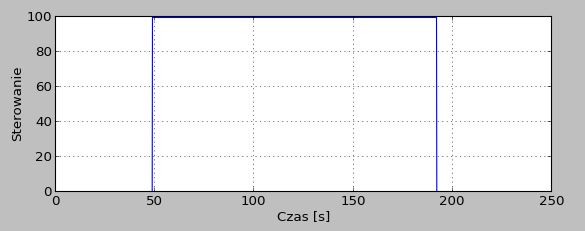
\includegraphics[width=\textwidth]{Grafika/ctrl_30_30_30-20_25_20-normalised}
    \caption{Przykład sterowania znormalizowanego. Źródło: własne.}
    \label{fig:ctrl-normalised-example}
\end{figure}

% wykomentowane, bo nieprawdziwe - poprawne działanie algorytmu skutkuje sterowaniem bang-bang
% Niestety, tak prosty algorytm ma swoje wady. Przede wszystkim nie umożliwia wyznaczania tylko dwóch czasów przełączeń w przypadku, gdy postać sterowania jest bardziej skomplikowana. To ogranicza stosowanie całej aplikacji tylko do przypadków, w których da się to zrobić, ponieważ założono, że wyższy jej poziom wysyła zawsze 2 czasy przełączeń.

%-------------------------------------------------
\subsection{Dokładność wyznaczania rozwiązania}
\label{sub:opt-dokladnosc}

Jedynym parametrem, który wyznacza dokładność wyznaczania rozwiązania przez pakiet JModelica.org jest relatywna tolerancja zbieżności programu IPOPT, którą można ustawić we właściwości \emph{IPOPTTolerance} (opisanej w sekcji \ref{sub:czesc-wyzsza-klasa}). Domyślną wartością jest $10^{-5}$, która jednak okazała się zbyt mała dla opisywanego problemu i prowadziła do błędów zbieżności i niemożliwości wyznaczenia odpowiedniego rozwiązania. Dobrano doświadczalnie wartość $10^{-3}$ ze względu na fakt, iż w tym przypadku niemożliwość wyliczenia sterowania optymalnego zdarzała się relatywnie rzadko. Obliczenia były prowadzone w centymetrach, więc taka wartość tolerancji odpowiada zmianie poziomu o 10 mikrometrów, która w przypadku omawianego układu zbiorników jest zupełnie wystarczająca.

Dodatkowo wartość wspomnianej właściwości \emph{IPOPTTolerance} jest również wykorzystywana do sprawdzenia, czy rozwiązanie zwrócone przez algorytm optymalizacyjny jest poprawne. Sprawdza się, czy odległość między wartościami końcowymi trajektorii systemu a stanem docelowym jest mniejsza niż wartość tej właściwości.

Opisane wyżej algorytmy inicjalizacji i optymalizacji pozwoliły osiągnąć zadowalające wyniki dla stanów znajdujących się blisko punktów równowagi układu. Nie przeprowadzono jednak pełnej analizy stanów osiągalnych systemu, a więc nie stwierdzono, czy brak poprawnego wyniku dla stanów docelowych bardziej oddalonych od punktów równowagi jest związany błędnym działaniem algorytmu, czy z faktem, iż te stany nie są osiągalne.
